% !TeX TXS-program:compile = txs:///lualatex

\documentclass[a4paper,11pt]{article}
\usepackage[breakable]{cp-base}
\graphicspath{{./graphics/}}
%variables
\donnees[%
	typedoc=CHAPITRE~,
	numdoc=5,
	classe=1\up{ère} 2M2,
	matiere={[SPÉ.MATHS]},
	annee=2021,
	titre={Probas conditionnelles, indépendance}
	]

%formatage
\author{Pierquet}
\title{\nomfichier}
\hypersetup{pdfauthor={Pierquet},pdftitle={\nomfichier},allbordercolors=white,pdfborder=0 0 0,pdfstartview=FitH}
%divers
\lhead{\entete{\matiere}}
\chead{\entete{\lycee}}
\rhead{\entete{\classe{} - Chapitre \thepart}}
\lfoot{\pied{\matiere}}
\cfoot{\logolycee{}}
\rfoot{\pied{\numeropagetot}}
\usepackage{setspace}

\begin{document}

\pagestyle{fancy}

\part{CH05 - Probabilités conditionnelles, indépendance}

\section{Rappels sur les probabilités}

\subsection{Généralités}

\begin{cdefi}[s]
L'ensemble de toutes les \textbf{issues} (ou \textbf{éventualités}) possibles d'une expérience aléatoire s'appelle l'\textbf{univers} de cette expérience aléatoire (souvent noté $\Omega$).

Un sous-ensemble de cet univers s'appelle un \textbf{événement}.
\end{cdefi}

\begin{cprop}
Une probabilité est toujours un nombre compris \textbf{entre 0 et 1}.

Dans le cas où toutes les issues sont \textbf{équiprobables} (c'est-à-dire qu'elles ont toutes les mêmes chances de se produire), la \textbf{probabilité} d'un événement est le quotient : \[p(A)=\dfrac{\text{nombre de cas favorables à } A}{\text{nombre de cas possibles dans l'univers}}.\]
\end{cprop}

\begin{chistoire}
\vspace{-0.22cm}
\lettrine[findent=.5em,nindent=0pt,lines=3,image,novskip=0pt]{huygens}{}\uline{Huygens} ($1629-1695$, $\vcenter{\hbox{
\includegraphics[height=0.5\baselineskip]{nl}}}$) et Cardan ($1501-1576$, $\vcenter{\hbox{
\includegraphics[height=0.5\baselineskip]{it}}}$) sont considérés comme les \og pères de la théorie des probabilités \fg. Cependant la mauvaise réputation de Cardan a fait pencher la paternité sur Pascal et Fermat. L'apparition de la notion de « risque », préalable à l'étude des probabilités, n'est apparue qu'au XII\up{e} siècle pour l'évaluation de contrats commerciaux avec le \textit{Traité des contrats} de Pierre de Jean Olivia.

Les idées se propagent en Italie et en France, Galilée écrit entre 1620 en 1718 son petit mémoire sur le jeu de dés intitulé \textit{Sopra le Scoperte de i Dadi} dans lequel il suppose l'équipossibilité des lancers. Cette notion d'équipossibilité se retrouve également, plus tard, dans la correspondance de Pierre de Fermat et dans celle de Pierre-Simon de Laplace.
\end{chistoire}

\subsection{Événements, calculs de probabilités}

\begin{cdefi}[s]
L'événement \textbf{contraire} (ou complémentaire) $\overline{A}$ d'un événement $A$ se réalise dès que $A$ ne se réalise pas:

\begin{center}
	\begin{tikzpicture}[scale=0.6]
		\draw (-3,-1.5) rectangle (3,1.5) ;
		\draw  (0,0) circle (2cm and 1cm) ;
		\fill[pattern=north west lines]  (0,0) circle (2cm and 1cm);
		\draw (0,-1.5) node[below] {\vphantom{$\overline{A}$}$A$} ;
	\end{tikzpicture}
	\hspace{0.5cm}
	\begin{tikzpicture}[scale=0.6]
		\draw (-3,-1.5) rectangle (3,1.5) ;
		\fill[pattern=north west lines]  (-3,-1.5) rectangle (3,1.5) ;
		\draw  (0,0) circle (2cm and 1cm);
		\fill[ForestGreen!15]  (0,0) circle (2cm and 1cm);
		\draw (0,-1.5) node[below] {$\overline{A}$} ;
	\end{tikzpicture}
\end{center}
\vspace{-0.2cm}
L'\textbf{intersection $A \cap B$ } (lire \og $A$ inter $B$ \fg) de deux événements est l'événement qui se réalise lorsque $A$ \textbf{ET} $B$ se réalisent \emph{simultanément}.

La \textbf{réunion} $A \cup B$ (lire \og $A$ union $B$ \fg) de deux événements est l'événement qui se réalise lorsque l'\emph{un au moins} des deux événements se réalise (l'un \textbf{OU} l'autre \textbf{OU} les deux).

\begin{center}
	\begin{tikzpicture}[scale=0.8]
		\draw (-3,-2) rectangle (5,1.5) ;
		\draw (2,-0.5) circle (2cm and 1cm);
		\draw (0,0) circle (2cm and 1cm);
		\draw (1,-2) node[below] {$A \cap B$} ;
		\clip (2,-0.5) circle (2cm and 1cm);
		\fill[pattern=north west lines]  (0,0) circle (2cm and 1cm);
	\end{tikzpicture}
	\hspace{0.5cm}
	\begin{tikzpicture}[scale=0.8]
		\draw (-3,-2) rectangle (5,1.5) ;
		\draw (2,-0.5) circle (2cm and 1cm);
		\draw (0,0) circle (2cm and 1cm);
		\fill[pattern=north west lines]  (0,0) circle (2cm and 1cm);
		\fill[pattern=north west lines]  (2,-0.5) circle (2cm and 1cm);
		\draw (1,-2) node[below] {$A \cup B$} ;
	\end{tikzpicture}
\end{center}
\end{cdefi}

\begin{cprop}[s]
Quels que soient les événements $A$ et $B$ :
\begin{itemize}
	\item $p(\overline{A})=1-p(A)$ ;
	\item $p(A \cup B)=p(A)+p(B)-p(A \cap B)$.\hfill{\red\itshape formule de la réunion}
\end{itemize}
\end{cprop}

\begin{cexemple}[ : test pharmaceutique]
Un laboratoire pharmaceutique a réalisé des tests sur 800 patients atteints d’une maladie. Certains sont traités avec le médicament A, d’autres avec le médicament B.

Le tableau ci-dessous présente les résultats de l’étude :
\begin{center}
	\begin{tabularx}{14cm}{|Y|Y|Y|Y|}
	\cline{2-4}
	\multicolumn{1}{c|}{}& Médicament A & Médicament B & Total \\
	\hline
	Guéri & 383 & 291 & 674 \\
	\hline
	Non Guéri & 72 & 54 & 126 \\
	\hline
	Total & 455 & 345 & 800 \\
	\hline
\end{tabularx}
\end{center} 
On choisit au hasard un patient testé, et on appelle $A$ l'événement \og le patient a été traité avec le médicament A \fg{} et $G$ : \og il est guéri \fg.
\begin{itemize}[leftmargin=*]
	\item $\overline{A}$ est l'événement : \og le patient a été traité avec le médicament B \fg{} ;
	\item $A \cap G$ est l'événement : \og le patient a été traité avec le médicament A \textbf{et} est guéri \fg{} ;
	\item $A \cup G$ est l'événement : \og le patient a été traité avec le médicament A \textbf{ou} est guéri \fg.
\end{itemize}
On a, de plus :
\begin{itemize}[leftmargin=*]
	\item $p(\overline{A})=1-p(A)=1-\dfrac{455}{800}=\dfrac{345}{800}$ ;
	\item $p(A \cap G)=\dfrac{383}{800}$ ;
	\item $p(A \cup G)=p(A)+p(G)-p(A \cap G)=\dfrac{455}{800}+\dfrac{674}{800}-\dfrac{383}{800}=\dfrac{746}{800}$.
\end{itemize}
\end{cexemple}

\section{Arbre pondéré, probabilités conditionnelles}

\subsection{Utilisation d'un arbre pondéré}

\begin{cdefi}
Un \textbf{arbre pondéré} est un arbre de choix dans lequel les \textbf{branches} n'ont pas toutes le même poids. Chacune des branches (primaire ou secondaire) est alors affectée d'un nombre précisant la \textbf{probabilité} de passer par ce chemin plutôt qu'un autre.

À la \textbf{racine} de l'arbre, on trouve toujours l'univers de l'expérience aléatoire, et à chaque \textbf{noeud} ou \textbf{feuille}, un événement.
\end{cdefi}

\begin{cillustr}
\begin{center}
	% Racine à Gauche, développement vers la droite
	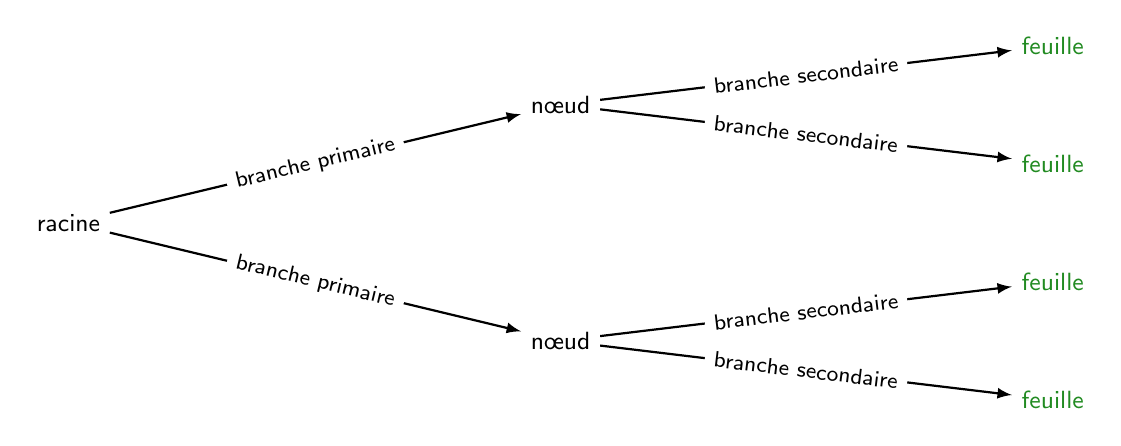
\begin{tikzpicture}[xscale=1,yscale=1]
		% Styles (MODIFIABLES)
		\tikzstyle{fleche}=[->,>=latex,thick]
		\tikzstyle{noeud}=[font=\sffamily\small]
		\tikzstyle{feuille}=[font=\sffamily\small,ForestGreen]
		\tikzstyle{etiquette}=[midway,fill=white,sloped,font=\sffamily\footnotesize]
		% Dimensions (MODIFIABLES)
		\def\DistanceInterNiveaux{5}
		\def\DistanceInterFeuilles{1.5}
		% Dimensions calculées (NON MODIFIABLES)
		\def\NiveauA{(0)*\DistanceInterNiveaux}
		\def\NiveauB{(1.25)*\DistanceInterNiveaux}
		\def\NiveauC{(2.5)*\DistanceInterNiveaux}
		\def\InterFeuilles{(-1)*\DistanceInterFeuilles}
		% Noeuds (MODIFIABLES : Styles et Coefficients d'InterFeuilles)
		\node[noeud] (R) at ({\NiveauA},{(1.5)*\InterFeuilles}) {\red racine};
		\node[noeud] (Ra) at ({\NiveauB},{(0.5)*\InterFeuilles}) {\blue nœud};
		\node[feuille] (Raa) at ({\NiveauC},{(0)*\InterFeuilles}) {feuille};
		\node[feuille] (Rab) at ({\NiveauC},{(1)*\InterFeuilles}) {feuille};
		\node[noeud] (Rb) at ({\NiveauB},{(2.5)*\InterFeuilles}) {\blue nœud};
		\node[feuille] (Rba) at ({\NiveauC},{(2)*\InterFeuilles}) {feuille};
		\node[feuille] (Rbb) at ({\NiveauC},{(3)*\InterFeuilles}) {feuille};
		% Arcs (MODIFIABLES : Styles)
		\draw[fleche] (R)--(Ra) node[etiquette] {branche primaire};
		\draw[fleche] (Ra)--(Raa) node[etiquette] {branche secondaire};
		\draw[fleche] (Ra)--(Rab) node[etiquette] {branche secondaire};
		\draw[fleche] (R)--(Rb) node[etiquette] {branche primaire};
		\draw[fleche] (Rb)--(Rba) node[etiquette] {branche secondaire};
		\draw[fleche] (Rb)--(Rbb) node[etiquette] {branche secondaire};
	\end{tikzpicture}
\end{center}
%:-+-+-+-+- Fin
\end{cillustr}

\begin{cexemple}[ : tirage dans une urne]
Un sac contient 20 boules rouges et 30 boules bleues. Chacune d'entre elles porte l'une des mentions \og Gagné \fg{} ou \og Perdu \fg. 15 boules rouges et 9 boules bleues sont gagnantes.

On tire au hasard une boule dans le sac, et on appelle $R$ l'événement \og La boule tirée est rouge \fg{} et $G$ \og La boule tirée est gagnante \fg. On peut schématiser cette expérience par l'arbre pondéré :	
	\begin{center}
		%urne
		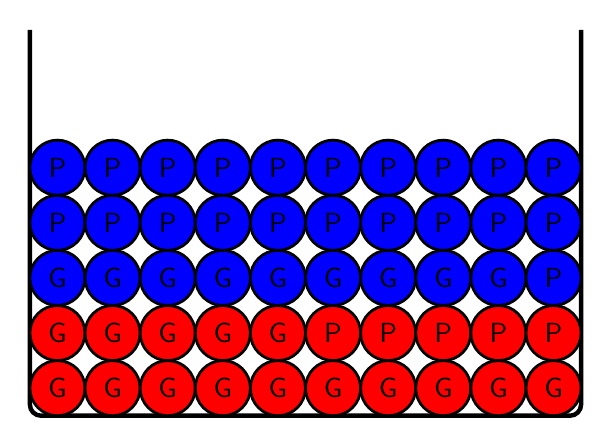
\begin{tikzpicture}[scale=0.7]
			%urne
			\draw[rounded corners,ultra thick] (0,7) -- (0,0) -- (10,0) -- (10,7) ;
			\foreach \centre in {0.5,1.5,...,9.5}
			\filldraw[line width=1pt,black,fill=red] (\centre,0.5) circle(0.5) node{\bfseries\white\sf G} ;
			\foreach \centre in {0.5,1.5,...,4.5}
			\filldraw[line width=1pt,black,fill=red] (\centre,1.5) circle(0.5) node{\bfseries\white\sf G} ;
			\foreach \centre in {5.5,6.5,...,9.5}
			\filldraw[line width=1pt,black,fill=red] (\centre,1.5) circle(0.5) node{\bfseries\white\sf P} ;
			\foreach \centre in {0.5,1.5,...,8.5}
			\filldraw[line width=1pt,black,fill=blue] (\centre,2.5) circle(0.5) node{\bfseries\white\sf G} ;
			\filldraw[line width=1pt,black,fill=blue] (9.5,2.5) circle(0.5) node{\bfseries\white\sf P} ;
			\foreach \centre in {0.5,1.5,...,9.5}
			\filldraw[line width=1pt,black,fill=blue] (\centre,3.5) circle(0.5) node{\bfseries\white\sf P} ;
			\foreach \centre in {0.5,1.5,...,9.5}
			\filldraw[line width=1pt,black,fill=blue] (\centre,4.5) circle(0.5) node{\bfseries\white\sf P} ;
		\end{tikzpicture}
		\hspace{0.5cm}
		% Racine à Gauche, développement vers la droite
		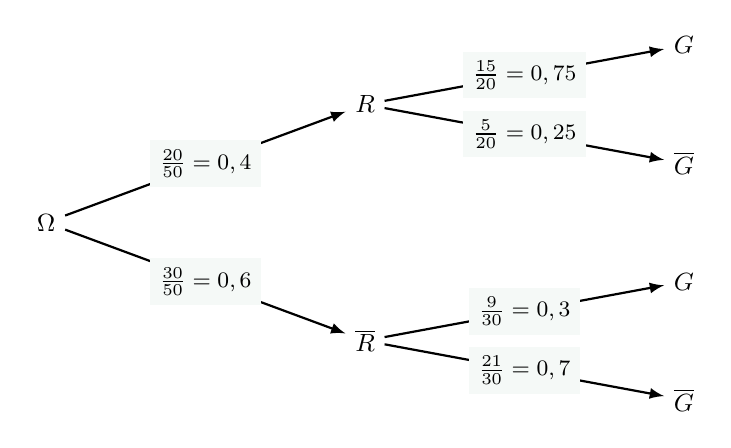
\begin{tikzpicture}[xscale=1,yscale=1]
			% Styles (MODIFIABLES)
			\tikzstyle{fleche}=[->,>=latex,thick]
			\tikzstyle{noeud}=[font=\sffamily\small]
			\tikzstyle{feuille}=[font=\sffamily\small]
			\tikzstyle{etiquette}=[midway,fill=SeaGreen!5,font=\sffamily\footnotesize]
			% Dimensions (MODIFIABLES)
			\def\DistanceInterNiveaux{3}
			\def\DistanceInterFeuilles{1.5}
			% Dimensions calculées (NON MODIFIABLES)
			\def\NiveauA{(0)*\DistanceInterNiveaux}
			\def\NiveauB{(1.35)*\DistanceInterNiveaux}
			\def\NiveauC{(2.7)*\DistanceInterNiveaux}
			\def\InterFeuilles{(-1)*\DistanceInterFeuilles}
			% Noeuds (MODIFIABLES : Styles et Coefficients d'InterFeuilles)
			\node[noeud] (R) at ({\NiveauA},{(1.5)*\InterFeuilles}) {$\Omega$};
			\node[noeud] (Ra) at ({\NiveauB},{(0.5)*\InterFeuilles}) {$R$};
			\node[feuille] (Raa) at ({\NiveauC},{(0)*\InterFeuilles}) {$G$};
			\node[feuille] (Rab) at ({\NiveauC},{(1)*\InterFeuilles}) {$\overline{G}$};
			\node[noeud] (Rb) at ({\NiveauB},{(2.5)*\InterFeuilles}) {$\overline{R}$};
			\node[feuille] (Rba) at ({\NiveauC},{(2)*\InterFeuilles}) {$G$};
			\node[feuille] (Rbb) at ({\NiveauC},{(3)*\InterFeuilles}) {$\overline{G}$};
			% Arcs (MODIFIABLES : Styles)
			\draw[fleche] (R)--(Ra) node[etiquette] {$\frac{20}{50}=0,4$};
			\draw[fleche] (Ra)--(Raa) node[etiquette] {$\frac{15}{20}=0,75$};
			\draw[fleche] (Ra)--(Rab) node[etiquette] {$\frac{5}{20}=0,25$};
			\draw[fleche] (R)--(Rb) node[etiquette] {$\frac{30}{50}=0,6$};
			\draw[fleche] (Rb)--(Rba) node[etiquette] {$\frac{9}{30}=0,3$};
			\draw[fleche] (Rb)--(Rbb) node[etiquette] {$\frac{21}{30}=0,7$};
		\end{tikzpicture}
	\end{center}
\end{cexemple}

\begin{cexercice}[ : test pharmaceutique]
Décrire la situation à l'aide d'un arbre pondéré.
\end{cexercice}

\begin{cthm}[s]
\vspace{-0.2cm}
\begin{itemize}[leftmargin=*]
	\item La somme des probabilités de toutes les branches partant d'un même noeud est toujours égale à 1.
	\item La probabilité d'un chemin est égale au produit des probabilités de toutes les branches qui le composent.
	\item La probabilité d'un événement est la somme des probabilités de tous les chemins qui mènent à cet événement.
\end{itemize}
\end{cthm}

\begin{cexemple}[ : tirage dans une urne]
La probabilité d'obtenir une boule rouge gagnante est $\tfrac{15}{50}=\tfrac{3}{10}=p(R \cap G)$.

\tabula{}Sur l'arbre, on retrouve bien  $0,4 \times 0,75 = 0,3$.

La probabilité d'obtenir une boule gagnante est $\tfrac{15+9}{50}=0,48$.

Sur l'arbre,  il y a deux chemins qui mènent à $G$ : le chemin $R \cap G$, de probabilité $0,3$ et le chemin $\overline{R} \cap G$ de probabilité $0,6 \times 0,3=0,18$. On retrouve bien $p(R \cap G)+p(\overline{R} \cap G)=0,3+0,18= 0,48=p(G)$.
\end{cexemple}

\begin{cexercice}[ : test pharmaceutique]
En utilisant l'arbre pondéré ci-dessus, déterminer $p(A)$, $p(B \cap G)$, $p(G)$, $p(\overline{G})$.
\end{cexercice}

\subsection{Probabilité conditionnelle}

\begin{cdefi}
Lorsqu'on construit un arbre pondéré comme ci-dessus, les probabilités inscrites sur les branches primaires sont des probabilités classiques, mais les probabilités inscrites sur les branches secondaires sont des \textbf{probabilités conditionnelles} : ce sont les probabilités d'arriver à ce nœud \emph{sachant que l'on vient de tel autre nœud}.

La probabilité conditionnelle que l'événement $B$ se réalise sachant que l'événement $A$ est réalisé  se note $p_A(B)$ (lire \og probabilité de $B$ sachant $A$ \fg) et, si $p(A) \neq 0$ :\[p_A(B)=\dfrac{p(A \cap B)}{p(A)}.\]
\end{cdefi}

\begin{crmq}[s]
\vspace{-0.2cm}
\begin{itemize}[leftmargin=*]
	\item Si $p(B) \neq 0$, on peut inverser les rôles de $A$ et $B$ dans la formule ci-dessus : $ p_B(A)=\dfrac{p(A \cap B)}{p(B)}$.
	\item Si les probabilités conditionnelles du type $p_A(B)$ sont en général données dans les énoncés, il arrive souvent qu'on doive inverser les conditions et calculer par exemple $p_B(A)$. C'est là que la formule est nécessaire.
\end{itemize}
\end{crmq}

\begin{cexemple}
$p_{R}(G)=0,75$ est la probabilité de tirer une boule gagnante \textit{sachant qu'elle est rouge}, autrement dit, la probabilité de tirer une boule rouge gagnante \textit{parmi les rouges}. Cette probabilité découle de la constitution de l'urne.

\smallskip

$p_{G}(R)$ ne figure pas dans l'arbre. C'est la probabilité d'avoir tiré une boule rouge \textit{sachant qu'elle est marquée gagnante}, autrement dit la probabilité de tirer une boule rouge gagnante \textit{parmi les boules gagnantes}. C'est moins naturel dans ce sens, puisqu'on voit la couleur de la boule avant d'y trouver la marque.

\hfill$p_{G}(R)=\frac{p(G \cap R)}{p(G)}=\frac{0,3}{0,48}=0,625$.\hfill~

On peut tout de même retrouver cette probabilité grâce à la constitution de l'urne : sur les $15+9=24$ boules gagnantes, il y en a 15 rouges et $\frac{15}{24}=0,625$.
\end{cexemple}

\begin{cexercice}[ : test pharmaceutique]
Calculer $p_G(A)$ de deux façons différentes : en utilisant l'arbre puis en utilisant le tableau à double entrée.
\end{cexercice}

\begin{cprop}[s]
$\bullet~~p(A \cap B)=p(A) \times p_A(B)$.\hfill{\red\itshape formule des probabilités composées}

$\bullet~~p_A(\overline{B})=1-p_A(B)$.
\end{cprop}

\begin{cdemoblanc}
\vspace{-0.2cm}
\begin{itemize}[leftmargin=*]
	\item C'est la formule que l'on utilise quand on dit que la probabilité d'un chemin est le produit de celles des branches qui le composent : \[p_A(B)=\dfrac{p(A \cap B)}{p(A)} \ssi p(A \cap B)=p(A) \times p_A(B).\]
	\item C'est la formule que l'on utilise quand on dit que la somme des probabilités des branches issues d'un même nœud est toujours égale à 1 : \vspace{-0.2cm}
	\begin{center}
		\begin{tikzpicture}[scale=0.5]
			\draw (2,-0.5) circle (2cm and 1cm);
			\draw (0,0) circle (2cm and 1cm);
			\draw (1,-1.5) node[below] {$A \cap B$} ;
			\clip (2,-0.5) circle (2cm and 1cm);
			\fill[pattern=north west lines]  (0,0) circle (2cm and 1cm);
		\end{tikzpicture}
		\hspace{0.5cm}
		\begin{tikzpicture}[scale=0.5]
			\fill[pattern=north west lines]  (0,0) circle (2cm and 1cm);
			\draw (2,-0.5) circle (2cm and 1cm);
			\fill[white]  (2,-0.5) circle (2cm and 1cm);
			\draw (0,0) circle (2cm and 1cm);
			\draw (1,-1.5) node[below] {$A \cap \overline{B}$} ;
		\end{tikzpicture}
	\end{center} \vspace{-0.2cm}
	En effet, la réunion de $A \cap B$ et $A \cap \overline{B}$ est égale à $A$ donc $p_A(\overline{B})+p_A(B)=\frac{p(A \cap \overline{B})}{p(A)}+\frac{p(A \cap B)}{p(A)}=\frac{p(A)}{p(A)}=1$.
\end{itemize}
\end{cdemoblanc}

\subsection{Formule des probabilités totales}

\begin{cdefi}[ : Partition de l'univers]
Soient $A_1, A_2, ..., A_n$ une liste d'évènements relatifs à une même expérience aléatoire.\\ On dit que ces événements réalisent une \textbf{partition} de l'univers si :
\begin{itemize}
	\item aucun de ces éléments n'est vide ;
	\item ils sont deux à deux disjoints (c'est-à-dire d'intersection vide) ;
	\item la réunion de tous ces événements recouvre l'univers tout entier.
\end{itemize}
\end{cdefi}

\begin{crmq}
En particulier, un événement $A$ et son événement contraire $\overline{A}$ forment une partition de $\Omega$.
\end{crmq}

\begin{cillustr}
Pour une partition à 4 éléments :
\begin{center}
	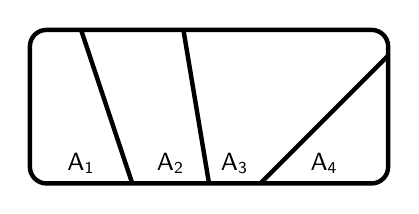
\begin{tikzpicture}[scale=0.65]
		\draw[rounded corners=6pt,ultra thick] (0,0) rectangle (7,3) ;
		%abscisses ligne du bas = 0 / 2 / 3.5 / 4.5 / 7 
		\draw[ultra thick] (1,3) -- (2,0) ;
		\draw[ultra thick] (3,3) -- (3.5,0) ;
		\draw[ultra thick] (4.5,0) -- (7,2.5) ;
		\tikzset{texte/.style={above,font=\blue\bfseries\small}}
		\draw (1,0) node[texte] {$\mathsf{A_1}$} ;
		\draw (2.75,0) node[texte] {$\mathsf{A_2}$} ;
		\draw (4,0) node[texte] {$\mathsf{A_3}$} ;
		\draw (5.75,0) node[texte] {$\mathsf{A_4}$} ;
	\end{tikzpicture}
\end{center}
\end{cillustr}

\begin{cthm}[ : Formule des probabilités totales]
Si les événements $A_1, A_2, ..., A_n$ réalisent une partition de l'univers, alors pour tout événement $B$ : \[p(B)=p(A_1 \cap B)+p(A_2 \cap B)+...+p(A_n \cap B).\]%
En particulier, pour tous événements $A$ et $B$ : \[p(B)=p(A \cap B) + p(\overline{A} \cap B).\]
\end{cthm}

\begin{cdemoblanc}[]
C'est la propriété qu'on utilise quand on dit que la probabilité d'un événement est la somme de toutes les probabilités des chemins qui mènent à cet événement. Elle vient du fait que les événements $A_1~\cap~B$, $A_2~\cap~B$,\ldots, $A_n~\cap~B$ sont deux à deux disjoints et recouvrent entièrement $B$.
\begin{center}
	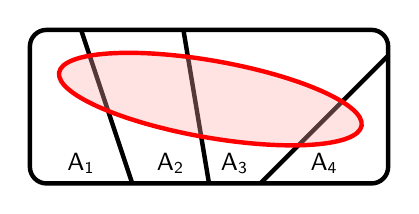
\begin{tikzpicture}[scale=0.65]
		\draw[rounded corners=6pt,ultra thick] (0,0) rectangle (7,3) ;
		\draw[ultra thick] (1,3) -- (2,0) ;
		\draw[ultra thick] (3,3) -- (3.5,0) ;
		\draw[ultra thick] (4.5,0) -- (7,2.5) ;
		\tikzset{texte/.style={above,font=\blue\bfseries\small}}
		\draw (1,0) node[texte] {$\mathsf{A_1}$} ;
		\draw (2.75,0) node[texte] {$\mathsf{A_2}$} ;
		\draw (4,0) node[texte] {$\mathsf{A_3}$} ;
		\draw (5.75,0) node[texte] {$\mathsf{A_4}$} ;
		%ellipse
		\draw[ultra thick,rotate around={-10:(3.5,1.5)},red,fill=red!33,fill opacity=0.33] (3.5,1.65) ellipse (3 and 0.75);
	\end{tikzpicture}
\end{center}
\end{cdemoblanc}

\begin{cillustr}
Sur un arbre, on peut visualiser et représenter différentes probabilités mises en jeu :
\begin{itemize}
	\item des \textcolor{purple}{conditionnelles} ;
	\item les \textcolor{ForestGreen}{composées} ;
	\item les \textcolor{red}{totales}.
\end{itemize}
\begin{center}
	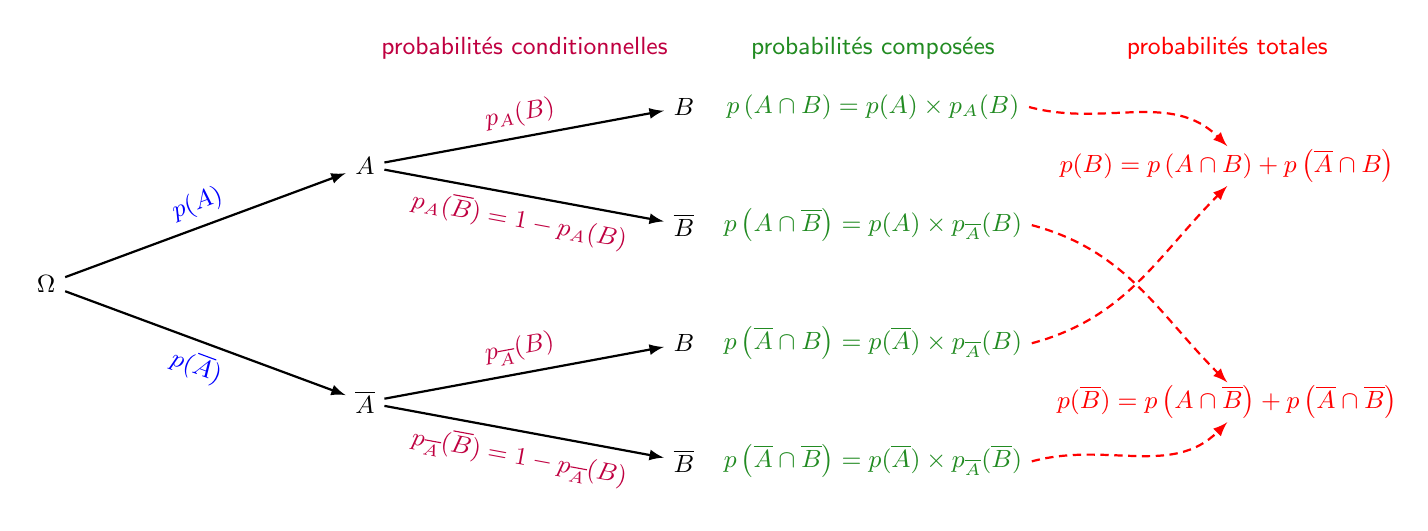
\begin{tikzpicture}[xscale=1,yscale=1]
		% Styles (MODIFIABLES)
		\tikzstyle{fleche}=[->,>=latex,thick]
		\tikzstyle{noeud}=[font=\small]
		\tikzstyle{feuille}=[ForestGreen,font=\small]
		\tikzstyle{etiquette}=[midway,sloped,font=\small]
		\tikzstyle{notice}=[font=\sffamily\small]
		% Dimensions (MODIFIABLES)
		\def\DistanceInterNiveaux{3}
		\def\DistanceInterFeuilles{1.5}
		% Dimensions calculées (NON MODIFIABLES)
		\def\NiveauA{(0)*\DistanceInterNiveaux}
		\def\NiveauB{(1.35)*\DistanceInterNiveaux}
		\def\NiveauC{(2.7)*\DistanceInterNiveaux}
		\def\NiveauD{(3.5)*\DistanceInterNiveaux}
		\def\NiveauE{(5)*\DistanceInterNiveaux}
		\def\InterFeuilles{(-1)*\DistanceInterFeuilles}
		% Noeuds (MODIFIABLES : Styles et Coefficients d'InterFeuilles)
		\node[noeud] (R) at ({\NiveauA},{(1.5)*\InterFeuilles}) {$\Omega$};
		\node[noeud] (Ra) at ({\NiveauB},{(0.5)*\InterFeuilles}) {$A$};
		\node[noeud] (Raa) at ({\NiveauC},{(0)*\InterFeuilles}) {$B$};
		\node[noeud] (Rab) at ({\NiveauC},{(1)*\InterFeuilles}) {$\overline{B}$};
		\node[noeud] (Rb) at ({\NiveauB},{(2.5)*\InterFeuilles}) {$\overline{A}$};
		\node[noeud] (Rba) at ({\NiveauC},{(2)*\InterFeuilles}) {$B$};
		\node[noeud] (Rbb) at ({\NiveauC},{(3)*\InterFeuilles}) {$\overline{B}$};
		% Arcs (MODIFIABLES : Styles)
		\draw[fleche,above] (R)--(Ra) node[etiquette,blue] {$p(A)$};
		\draw[fleche,above] (Ra)--(Raa) node[etiquette,purple] {$p_{A}(B)$};
		\draw[fleche,below] (Ra)--(Rab) node[etiquette,purple] {$p_{A}(\overline{B})=1-p_{A}(B)$};
		\draw[fleche,below] (R)--(Rb) node[etiquette,blue] {$p(\overline{A})$};
		\draw[fleche,above] (Rb)--(Rba) node[etiquette,purple] {$p_{\overline{A}}(B)$};
		\draw[fleche,below] (Rb)--(Rbb) node[etiquette,purple] {$p_{\overline{A}}(\overline{B})=1-p_{\overline{A}}(B)$};
		%feuilles
		\node[feuille] (F1) at ({\NiveauD},{(0)*\InterFeuilles}) {$p\left(A \cap B \right) = p(A) \times p_A(B)$};
		\node[feuille] (F2) at ({\NiveauD},{(1)*\InterFeuilles}) {$p\left(A \cap \overline{B} \right) = p(A) \times p_{\overline{A}}(B)$};
		\node[feuille] (F3) at ({\NiveauD},{(2)*\InterFeuilles}) {$p\left(\overline{A} \cap B \right) = p(\overline{A}) \times p_{\overline{A}}(B)$};
		\node[feuille] (F4) at ({\NiveauD},{(3)*\InterFeuilles}) {$p\left({\overline{A}} \cap \overline{B} \right) = p(\overline{A}) \times p_{\overline{A}}({\overline{B}})$};
		%totales
		\node[feuille,red,inner sep=1pt] (T1) at ({\NiveauE},{(0.5)*\InterFeuilles}) {$p(B)=p\left(A \cap B \right) +p\left(\overline{A} \cap B \right)$};
		\node[feuille,red,inner sep=1pt] (T2) at ({\NiveauE},{(2.5)*\InterFeuilles}) {$p(\overline{B})=p\left(A \cap \overline{B} \right) +p\left(\overline{A} \cap \overline{B} \right)$};
		%fléches dashed
		\draw[fleche,densely dashed,red] (F1.east) to [out=-15,in=135] (T1.north) ;
		\draw[fleche,densely dashed,red] (F3.east) to [out=15,in=-135] (T1.south) ;
		\draw[fleche,densely dashed,red] (F2.east) to [out=-15,in=135] (T2.north) ;
		\draw[fleche,densely dashed,red] (F4.east) to [out=15,in=-135] (T2.south) ;
		%notices
		\draw[notice,purple] ({(0.5)*\NiveauB+(0.5)*\NiveauC},{(-0.5)*\InterFeuilles}) node {probabilités conditionnelles} ;
		\draw[notice,ForestGreen] ({\NiveauD},{(-0.5)*\InterFeuilles}) node {probabilités composées} ;
		\draw[notice,red] ({\NiveauE},{(-0.5)*\InterFeuilles}) node {probabilités totales} ;
	\end{tikzpicture}
\end{center}
\end{cillustr}

\newpage

\section{Indépendance}

\subsection{Événements indépendants}

\begin{cdefi}[ - Propriété]
On dit que deux événements  de probabilités non nulles sont \textbf{indépendants} s'ils vérifient l'une ou l'autre des propriétés ci-dessous, qui sont équivalentes : \[ p(A \cap B)=p(A) \times p(B) \ssi p_A(B)=p(B) \ssi p_B(A)=p(A).\]%
Autrement dit, la réalisation d'un événement n'influence pas la probabilité de l'autre.
\end{cdefi}

\begin{cdemoblanc}
En effet, a priori on a $p(A \cap B)=p(A) \times p_A(B) $ donc si les événements sont indépendants :

\tabula{}$p(A \cap B)=p(A) \times p(B) = p(A) \times p_A(B) $ et donc si $p(A) \neq 0$, on retrouve bien $ p(B) =  p_A(B) $. 
\end{cdemoblanc}

\begin{cexemple}
On tire une carte au hasard dans un jeu de 32 cartes. On appelle $C$ l'événement \og Obtenir un cœur \fg{} et $D$ \og Obtenir une dame \fg. $C \cap D$ est alors \og Obtenir la dame de cœur \fg.

\begin{center}
	\def\hauteur{1}
	\poker{7C}{\hauteur}~\poker{8C}{\hauteur}~\poker{9C}{\hauteur}~\poker{10C}{\hauteur}~\poker{VC}{\hauteur}~\poker{DC}{\hauteur}~\poker{RC}{\hauteur}~\poker{AC}{\hauteur}~\poker{DK}{\hauteur}~\poker{DP}{\hauteur}~\poker{DT}{\hauteur}
\end{center}

\smallskip

$\bullet~~p(C)=\frac{8}{32}=\frac{1}{4}$ et $p(D)=\frac{4}{32}=\frac{1}{8}$ et
$p(C \cap D)=\frac{1}{32}$ et $\frac{1}{4} \times \frac{1}{8} = \frac{1}{32}$ donc $C$ et $D$ sont indépendants. 

\smallskip

On a aussi $p_C(D)=p(D)$, c'est-à-dire que la probabilité d'obtenir une dame parmi les cœurs est la même que celle d'obtenir une dame parmi toutes les cartes : $\frac{1}{8}$ .

\medskip

Maintenant, si on rajoute deux jokers dans le jeu :

\smallskip

$\bullet~~p(C)=\frac{8}{34}$ et $p(D)=\frac{4}{34}$ et
$p(C \cap D)=\frac{1}{34}$ et $p(C) \times p(D) = \frac{8 \times 4}{34 \times 34} \neq p(C \cap D)$ donc $C$ et $D$ pas indépendants. 

\smallskip

De même, $p_C(D)=\frac{1}{8}$ mais $p(D)= \frac{4}{34}$ et ces probabilités ne sont plus égales.
\end{cexemple}

\begin{cprop}
Si $A$ et $B$ sont indépendants, alors $\overline{A}$ et $B$ sont indépendants.
\end{cprop}

\begin{cdemoblanc}
$p(\overline{A} \cap B)+p(A \cap B)=p(B)$ d'après la formule des probabilités totales, donc, si $A$ et $B$ sont indépendants, \\ $p(\overline{A} \cap B)+p(A) \times p(B) = p(B)$ et ainsi $p(\overline{A} \cap B)=p(B)-p(A) \times p(B) = p(B)(1-p(A))=p(B)\times p(\overline{A})$.
\end{cdemoblanc}

\subsection{Expériences indépendantes}

\begin{cdefi}
Lorsque deux expériences aléatoires se succèdent et que les résultats de la première n'ont aucune influence sur les résultats de la seconde, on dit qu'il s'agit d'une \textbf{succession d'épreuves indépendantes}.
\end{cdefi}

\begin{cexemple}
On tire au hasard successivement deux cartes dans un jeu de 32 cartes.

Si on remet la carte avant le deuxième tirage, les conditions initiales sont identiques, donc on peut considérer que les deux tirages sont indépendants.

Si on ne remet pas la carte, la constitution du paquet dépend de la première carte tirée, donc les expériences ne sont pas indépendantes.
\end{cexemple}


\begin{cprop}[ (admise)]
Lorsque deux épreuves sont indépendantes, la probabilité d'un couple de résultats est égale au produit des probabilités de chacun d'eux.
\end{cprop}

\begin{cexemple}
On lance deux fois de suite un dé cubique.

La probabilité d'obtenir un double 5 est $\frac{1}{6} \times \frac{1}{6}$.
\end{cexemple}

\vfill{}

\begin{chistoire}[ - Anecdote]
\begin{minipage}{0.33\linewidth}
	\begin{center}
		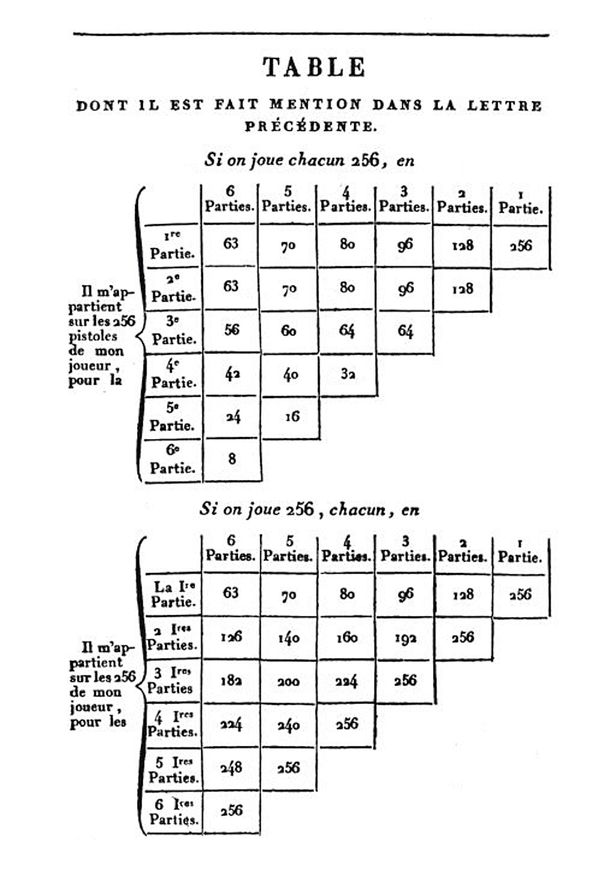
\includegraphics[width=4cm]{chap05_table}
	\end{center}
\end{minipage}\hfill
\begin{minipage}{0.65\linewidth}
\begin{center}
	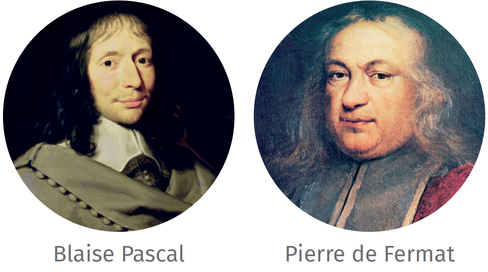
\includegraphics[height=1.25cm]{chap05_pascalfermat}
\end{center}
\setstretch{0.7}{\policeqtcanaithtype\scriptsize Le \textit{chevalier de Méré} (17\up{e} siècle) était un joueur et souhaitait connaître les stratégies amenant à un plus grand nombre de succès. Il soumet ce problème : « Deux joueurs misent chacun 32 pistoles dans un jeu en trois manches gagnantes. La partie est interrompue alors que le premier joueur a remporté deux manches et le second une seule. Quel doit être alors le gain de chacun des deux joueurs ? » Pascal et Fermat relèvent le défi et on retrouve les réponses dans leurs échanges épistolaires.
 Le problème décrit par le chevalier de Méré est un problème historique que l’on trouve déjà dans le \textit{Summa de Arithmetica} de Luca Pacioli (1494). Pascal et Fermat sont les premiers à y apporter une solution mathématique généralisable.\\ C’est cependant le Hollandais Christiaan Huygens qui publie en 1657 le premier traité mathématique consacré aux probabilités : \textit{Tractatus de Rariociniis in Alea Ludo}. De nos jours, les probabilités constituent une partie très importante des mathématiques.}
\end{minipage}

~\hfill{}{\tiny Source : \textit{LeLivreScolaire}}
\end{chistoire}

\begin{chumour}
	\vspace{-0.2cm}
	\begin{center}
		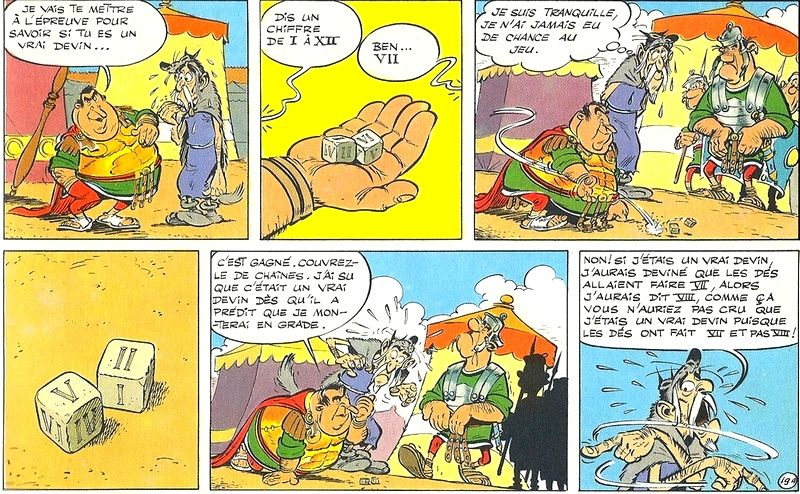
\includegraphics[width=8cm]{chap05_devin}
		
		{\tiny Source : \textit{Astérix}, Uderzo \& Goscinny}
	\end{center}
\end{chumour}

\end{document}